\documentclass[11pt, twocolumn]{article}
\usepackage[margin=1in]{geometry}
\usepackage{microtype}
\usepackage{float}
\usepackage{flushend}
\usepackage{graphicx, setspace, mathptmx, titling} 
\usepackage{xspace}
\usepackage{enumitem}
\usepackage{booktabs} 
\usepackage{siunitx}

\title{Evaluation Linux Pipes as an IPC Mechanism}
\author{Patrick DeCabooter}
\date{}

\newcommand{\cgt}{\texttt{clock\_gettime}\xspace}
\newcommand{\gtod}{\texttt{gettimeofday}\xspace}
\newcommand{\pipe}{\texttt{pipe}\xspace}
\newcommand{\pipes}{\texttt{pipes}\xspace}

\begin{document}

\maketitle

\section{Introduction}
Inter-process communication (IPC) is a critical trade-off of virtual memory systems.
Before we had virtual memory, IPC was as simple as passing the pointer to the data between the two processes. 
However, when each process is sand-boxed in its own virtual memory environment, the process sending
the data has no way to reason about the addresses of the process receiving the data, and 
vice-versa. Unfortunately for IPC, virtual memory has countless benefits and is here
to stay.

Enter \pipes, the first and oldest method of IPC chosen by the Linux kernel. 
Linux \pipes create one-way channels between two processes. They contain two file descriptors,
one to write to, and one to read from. In between writes and reads, the transfer payload 
is stored in a kernel-space buffer.

In this report we will:
\begin{enumerate}[label=(\arabic*), nosep]
  \item Evaluate the precision of two Linux timers that will be used for measurement.
  \item Measure the minimum latency of \pipes when sending various payload sizes.
  \item Measure the average throughput of \pipes when continuously sending large payloads. 
\end{enumerate}

\section{Linux Timers}
We tested two types of timers for our experiments. 
The first timer, provided by the header \texttt{time.h}, is \cgt.
We chose \texttt{CLOCK\_MONOTONIC} as the clock to use for \cgt due 
to it having guaranteed monotonicity and being system-wide. 
\cgt provides nanosecond precision.
The second timer, provided by the header \texttt{sys/time.h}, is \gtod.
\gtod finds the time by measuring the clock cycles since the last kernel epoch.
\gtod provides microsecond precision.
\gtod is a much older clock. By the time cpu-cycles were able to measure nanoseconds,
\gtod's interface was already locked-in to microseconds. \cgt was introduced as an api to replace \gtod.
In order to have similar units, we scaled \gtod up to nanoseconds instead of scaling \cgt
down to microseconds. 
We chose to do it this way since it would take advantage of \cgt's
increased accuracy and give us more intuitive numbers for figures.

\section{Linux Pipes}
When data moves between processes in a \pipe, it is not as simple as the other process reading it out of virtual memory.
First, the data must be sent by \texttt{write} and cross the system call barrier to enter kernel-space memory.

and use the \pipe writing file descriptor as an address. Then, the reader must call the \texttt{read} 
system call and wait to copy the data from kernel-space memory into a buffer in the user-space of that process.

\section{Evaluation}

\subsection*{Clock Precision}
To evaluate the accuracy of these two timers, we decided to measure accuracy against
\texttt{sleep} from the header \texttt{unistd.h} and measure the smallest measurable time.
To measure against \texttt{sleep}, we started the timer, called \texttt{sleep(5)}, then 
measured the final time to get the difference. We did this five times in a loop for each timer,
and took the minimum result. To measure the smallest measurable time, we had to compromise to
instead find the smallest measurable time for \gtod since it measures in microseconds instead of 
nanoseconds. To make a one microsecond delay, we summed the numbers from 0 to 99 in a loop. 
We did this this 10 times and took the minimum result. We used minimums as our metric for both
tests since we wanted to find the highest fidelity possible if our machine was running perfectly.

\begin{figure}[t]
  \centering
  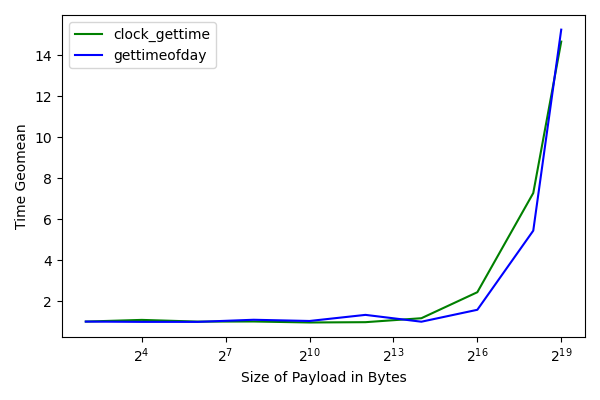
\includegraphics[width=\columnwidth]{pipe_latency}
  \caption{Latency of \pipe across different payload sizes. The x-axis shows
  payload size in bytes on a log base-2 scale. The y-axis shows the geometric mean relative
  to the smallest payload size of 4 bytes.}
  \label{fig:pipe_latency}
\end{figure}

\subsection*{Pipe Latency}
We tested 10 different payload
sizes and measured the time from payload send to acknowledgement acquisition. To construct our 
experiment, we had two processes. The parent process forked itself at the start of execution.  The child enters a loop where it waits for the parent to send data then acknowledges the request.
The parent sends each payload size 10 times and calculates the minimum latency for each size. 
The payload sizes we used were: 4, 16, 64, 256, 1K, 4K, 16K, 64K, 256K, and 512K bytes. We ran
both experiments using the \cgt and \gtod timers. We hypothesis that the majority of the latency of the \pipes will be from 
context switching and copying the memory in these system calls. We will test this by compiling as a static binary and using the
\texttt{time} and \texttt{perf} utilities to measure time spent in user-space and kernel-space.

The hypothesis that most of the time would be spent inside of the system calls was accurate to the
measured results. Using the \texttt{time} utility showed that out of $0.051$ seconds spent on the benchmark,
$0.001$ second was spent in user-space and $0.047$ seconds were spent in kernel-space. To further prove this
hypothesis, the \texttt{perf} utility recorded that the parent process spent $66.66\%$ of the runtime in \texttt{\_\_libc\_read} 
and $33.33\%$ of the runtime getting the time from the clock in \texttt{\_\_vdso\_clock\_gettime}.

\subsection*{Pipe Throughput}


\section{Conclusion}
Fart

\section{Computer Specification}
\begin{table}[htbp]
\centering
\begin{tabular}{ll}
  \toprule
  Component & Specification \\
  \midrule
  Computer Model & HP - Elite Dragonfly G4 \\
  Architecture & x86-64 \\
  Intel Core i7-1355U & 10 Cores / 12 Logical Processors \\
  RAM & 32 GiB / 4800 MT/s \\
  NVMe SSD & 1 TB \\
  Virtualization & WSL2 \\
  OS & Ubuntu 24.04.3 LTS \\
  Kernel & Linux 6.6.87.2-microsoft-standard-WSL2 \\
  Compiler & gcc version 13.3.0 \\
  \bottomrule
\end{tabular}
\end{table}


\end{document}